\documentclass[10pt,letter]{article}
\usepackage{amsmath}
\usepackage{amssymb}
\usepackage{graphicx}
\usepackage{setspace}
\onehalfspacing
\usepackage{fullpage}
\newcommand{\R}{\mathbb{R}}	
\newcommand{\inner}{\langle\cdot,\cdot\rangle}
\newcommand{\inr}[2]{\langle #1, #2\rangle}
\newcommand\norm[1]{\left\lVert#1\right\rVert}

\graphicspath{ {images/} }

\begin{document}


\title{CS142 Homework Set \#4 Solutions}

\author{Timur Kuzhagaliyev}

%\date{24th October, 2017}
 
\maketitle 

\section*{Problem 1}

Proof that concurrency is transitive:

\begin{align*}
& ( A\; \lVert\; B ) \land ( B\; \lVert\; C )
\\ \equiv \quad & \qquad \{\ \textrm{Definition of concurrency twice}\ \} \\
& ((\neg (A \rightarrow B) \land \neg (B \rightarrow A)) \land ((\neg (B \rightarrow C) \land \neg (C \rightarrow B))
\\ \equiv \quad & \qquad \{\ \textrm{De Morgan's law twice}\ \} \\
& \neg( (A \rightarrow B) \lor (B \rightarrow A)) \land \neg( (B \rightarrow C) \lor (C \rightarrow B))
\\ \equiv \quad & \qquad \{\ \textrm{De Morgan's law once}\ \} \\
& \neg ( (A \rightarrow B) \lor (B \rightarrow A) \lor (B \rightarrow C) \lor (C \rightarrow B) )
\\ \equiv \quad & \qquad \{\ \textrm{Definition of $\rightarrow$ 4 times}\ \} \\
& \neg ( (\neg A \lor B) \lor (\neg B \lor A) \lor (\neg B \lor C) \lor (\neg C \lor B) )
\\ \equiv \quad & \qquad \{\ \textrm{$\lor$ is associative and commutative}\ \} \\
& \neg ( \neg A \lor C \lor \neg C \lor A \lor B \lor \neg B \lor \neg B \lor B )
\\ \Rightarrow \quad & \qquad \{\ \textrm{$B \lor \neg B \equiv true$ and $true$ is the identity of $\lor$}\ \} \\
& \neg (\neg A \lor C \lor \neg C \lor A )
\\ \equiv \quad & \qquad \{\ \textrm{Definition of $\rightarrow$ 2 times}\ \} \\
& \neg (( A \rightarrow C ) \lor ( C \rightarrow A ))
\\ \equiv \quad & \qquad \{\ \textrm{De Morgan's law once}\ \} \\
& \neg ( A \rightarrow C ) \land \neg ( C \rightarrow A )
\\ \equiv \quad & \qquad \{\ \textrm{Definition of concurrency once}\ \} \\
& ( A\; \lVert\; C )
\end{align*}

\pagebreak

\section*{Problem 2}

Solution to problem 2:

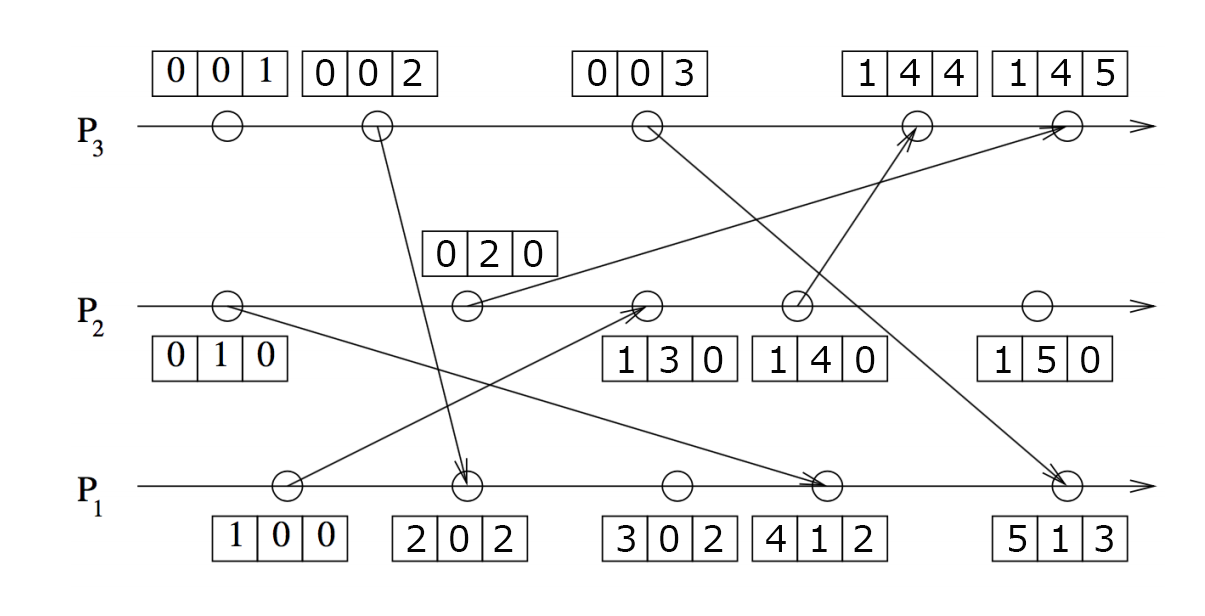
\includegraphics[width=\textwidth,height=\textheight,keepaspectratio]{hw4_problem2}

\section*{Problem 3}

\paragraph{a)} The algorithm is correct. We're told that the OS can observe the state of the entire distributed system at any point in time, including both agent and channel states. Note that the system terminates when all channels are empty and and all agents are idle, and we also know that $\textbf{stable}(terminated)$.

By definition of our algorithm, once the OS observes that $terminated$ holds (which can happen at most $T$ units of time after actual termination), it will set the value of $claim\_terminated$ to $true$. Clearly, the progress property holds as $terminated \leadsto claim\_terminated$.

Denote the point in time when the OS observes $terminated = true$ as $T_0$. By definition of the algorithm, $claim\_terminated$ is false up until $T_0$, so by definition of implication $claim\_terminated \Rightarrow terminated$ is $true$ up until $T_0$. At and after $T_0$, $terminated$ is $true$ (by definition of $T_0$) and OS sets $claim\_terminated$ to $true$ also. Since $terminated$ is stable, it will remain $true$, and by definition of our algorithm so will $claim\_terminated$. This means that at and after $T_0$ the predicate $claim\_terminated \Rightarrow terminated$ still evaluates to $true$. Since together time intervals before and after $T_0$ make up the whole time domain, $claim\_terminated \Rightarrow terminated$ always holds and hence is invariant. Therefore the safety property is satisfied.

By the two points above, the algorithm is correct.

 \paragraph{b)} Note that the total number of messages sent or received by an agent cannot be negative, and cannot decrease (since it's impossible to unsend/unreceive a message in our model). Note also that in our model the messages can't appear out of nowhere, so for agent to receive a message means that some other agent had to send it.
 
We know that each agent increments the number of sent messages by one when it sends a message, and increments the number of received messages by one when it receives a message. By the point above, it should be clear that for an agent to be able to increment their received messages counter, some other agent must have incremented their sent messages counter. If you take into account the fact that agents can go idle at any arbitrary point in time and the fact that messages are not necessarily delivered instantly (i.e. there might be messages in flight when an agent sends a message to the OS), it should be clear that $\sum\limits_{r} r.count\_received \leq \sum\limits_{r} r.count\_sent$. Moreover, $\sum\limits_{r} r.count\_received \leq \sum\limits_{r} r.count\_sent$ is invariant.

We also know that each message eventually gets delivered, so eventually each increment to $count\_sent$ gets balanced out by an increment to $count\_received$. Now, assume that OS has received at least one message from each agent and sees (for the first time) that the following statement holds:

\[
\sum\limits_{r} r.count\_received = \sum\limits_{r} r.count\_sent
\]

Clearly, if this is the first time this statement holds, $claim\_terminated$ must have been $false$ up until now, which implies $claim\_terminated \Rightarrow terminated$ was $true$. We know that we received at least one message from every agent, meaning that every agent has gone idle at least once. In our model, the agent can only be awoken when it receives a message - meaning that someone else had to send the message in the first place. Since we observe $\sum\limits_{r} r.count\_received = \sum\limits_{r} r.count\_sent$, we can conclude that there are no messages in transit and all agents are idle. This can be shown by contradiction - assume that there still exists an agent that is currently active. Since we know that all agents went idle at least once, they must've received a message to wake up. BUT since the agent in our assumption is still active, it did not report the amount of messages it has received, hence $\sum\limits_{r} r.count\_received$ should be strictly less than $\sum\limits_{r} r.count\_sent$, contradicting our observation. All channels should be empty too, since the counters imply that all messages that were sent were received. Hence we know that the system has terminated and will remain terminated because $\textbf{stable}(terminated)$. Now our $claim\_terminated$ will become and remain $true$ by definition of the algorithm, implying that $claim\_terminated \Rightarrow terminated$ holds after observation too. Clearly, safety property is satisfied as $claim\_terminated \Rightarrow terminated$ is invariant.

We can show that the progress property is satisfied. Initially, all agents are active so the system is clearly not terminated. The system would be terminated when all agents are idle and all channels are empty, which would imply that each agent would have to transit from active to the idle state. This transition, by definition of our algorithm, would cause the agents to send OS a message with their counters. That is, when the system will terminate, OS would have received a message from every single agent. As explained above, the last agent to go idle without sending any messages would cause the statement $\sum\limits_{r} r.count\_received = \sum\limits_{r} r.count\_sent$ to become true. Above we've also shown by contradiction that these indeed would have to be the case for the last agent going idle. We have shown that when the program terminates, OS would have received at least one message from each agent and has also seen the statement $\sum\limits_{r} r.count\_received = \sum\limits_{r} r.count\_sent$ holds, hence settings $claim\_terminated$ to true. This confirms that progress property, $terminated \leadsto claim\_terminated$, also holds with this algorithm.

 \paragraph{c)} \textbf{Proving invariant}: We know that $claim\_terminated$ is initially false and will remain false until OS observes all necessary properties. Denote the moment when OS sets $claim\_terminated$ to true as $T_0$. Clearly, before $T_0$ $claim\_terminated \Rightarrow terminated$ holds by definition of implication.

We know that $terminated$ is stable, so if we can show that at $\tau = T_0$ the conditions observed by the OS indeed show that the system has terminated, we can infer that the system will remain terminated. We can prove that by contradiction. We know that at time $\tau$ (with respect to each agent's individual logical clock) all agents were inactive. The only thing that could activate them afterwards was an incoming message. Assume there was indeed an agent that got activated after our observation. For this to be possible, someone must have sent a message to activate, and there are two ways this could happen:

\begin{itemize}
\item The message was sent before time $\tau$. If the message was sent before $\tau$, one of the agents would have incremented their sent message counter by one. Since the message would still be in flight at $\tau$, the total sum of all received messages would be 1 count below the total sum of all sent messages, which contradicts the observation of the OS.
\item The message was sent after time $\tau$. For this to be possible there must be at least one active agent after $\tau$, which is not the case as seen in our observation.
\end{itemize}

Hence, by contradiction, no agent can become active after $T_0$ and all channels must be empty. This implies that the system has terminated, and $claim\_terminated \Rightarrow terminated$ holds. Therefore $claim\_terminated \Rightarrow terminated$ is invariant. Note that we used the idea explained in part b), namely the $\sum\limits_{r} r.count\_received \leq \sum\limits_{r} r.count\_sent$ invariant.

\textbf{Showing progress}: We're given that the logical clock on each agent increments eventually, and each agent reports its state to OS after every interval $T$ with respect to its own clock. Let $T_{max}$ be the longest of intervals $T$ of all agents, in absolute time units. Since the agents report their progress periodically, once the system terminates, we know that OS will see the state of all agents after termination at most after $T_{max}$ absolute units of time after the actual termination occurred.

When $terminated$ holds, we know that all agents are idle and all channels are empty. It is clear that agents will report their states as idle, what satisfies one property of OS termination claim. Since there are no messages in channels, all sent messages must have been received, so total sum of sent messages is equal to total sum of received messages, what satisfies the second property of OS termination claim. Hence OS will set the $claim\_terminated$ to true. This shows that the algorithm satisfies the progress property $terminated \leadsto claim\_terminated$.

By the 2 points above, the algorithm is correct.

\end{document}